\documentclass[11pt]{article}
\usepackage[letterpaper,margin=0.9in]{geometry}
\usepackage{amsmath,amssymb,booktabs,graphicx,microtype}
\usepackage[hidelinks]{hyperref}
\urlstyle{same}
\makeatletter\let\tableinput\@@input\makeatother
\setlength{\parskip}{.32em}
\setlength{\parindent}{0pt}
\newcommand{\MSE}{\mathrm{MSE}}
\newcommand{\mn}{\mathrm{MN}}
\newcommand{\FigureProvenance}{}
\title{When a single training subset sets the peak of a minimum-norm learning curve}
\author{Yunjie Guo \qquad Hanqing Yang\\[2pt]
\small Independent Researcher, Suzhou, China\\
\small Correspondence: \href{mailto:hanqing.yang189@gmail.com}{hanqing.yang189@gmail.com}}
\date{}
\begin{document}
\maketitle
\begin{abstract}
The peak of an empirical learning curve can depend on how a solver defines numerical rank. We compare minimum-norm least squares, cross-validated ridge and principal components regression on artist-disjoint music data and an exact-feature-grouped materials holdout. Each comparison uses 100 training permutations at 15 sample sizes. Ridge has the lowest mean squared error of the three estimators at every size. On materials, one training subset accounts for 99.92\% of minimum-norm loss at the mean curve's peak, $n=73$ with 81 features. In a post-hoc recomputation, imposing a relative singular-value cutoff of $10^{-12}$ changes the fitted rank in just five of 1,500 subsets. The mean peak moves to $n=83$, while the median peak remains at $n=81$. Exact rank certificates on the recorded decimal features show that the worst subset has centered rank 71. The default fit retained all 71 directions. Thus a meaningful change in the peak can result from discarding an algebraically nonzero direction. The findings quantify how numerical regularization and the choice of loss summary affect the reading of a finite-benchmark learning curve.

\end{abstract}

\section{What sets the peak?}
A peak in a learning curve is often interpreted as evidence that the number of examples has reached the number of fitted parameters. In isotropic linear models this interpretation has a precise basis. For ridgeless least squares, risk can diverge as the aspect ratio approaches one \cite{hastie}. Optimally tuned ridge can mitigate double descent \cite{nakkiran}. These results leave a practical question for an investigator looking at a finite collection of training sets: would the same training size appear most difficult if almost every fitted model were unchanged, but the solver discarded a few additional singular directions?

We study this question using two completed comparisons of minimum-norm regression, ridge regression and principal components regression (PCR). The estimated response is the expected error over training subsets on a particular held-out set. At each size the same subsets and test rows are used for all three fits. The music benchmark supplies a reference with an artist-disjoint test set. In the materials benchmark, the largest arithmetic mean occurs well below the nominal interpolation boundary. We trace this discrepancy from the shape of the learning curve to individual fits, then recompute their predictions after changing the singular-value cutoff. An exact-arithmetic rank check asks how much of the apparent degeneracy is already present in the \emph{recorded decimal features}.

Classical truncated SVD explains how removing weak directions can change a solution \cite{hansen}. High-dimensional analyses also distinguish conditions favoring ridge and PCR under covariate shift \cite{tang}. Our contribution is an empirical account of which fits move a measured peak, by how much, and whether the change reaches the typical training subset. It uses fixed feature dimension and two distinct holdout designs.

\section{Benchmark comparisons}
\textbf{Sampling and endpoints.} YearPredictionMSD has 90 audio features. The official artist-disjoint partition puts the first 463,715 songs in the source pool and the last 51,630 in the holdout \cite{year}. The Superconductivity data contain 81 materials descriptors per row \cite{super}. Grouping the 21,263 rows by their complete float64 feature vector yields 15,170 groups. A seeded permutation allocates 12,136 groups (16,871 rows) to training and 3,034 groups (4,392 rows) to the holdout. The group assignment uses features alone. The materials protocol was frozen after the music results were available and before the materials outcomes were opened.

In each benchmark 100 stored seeds generate 100 permutations of the source row indices. The first $n$ rows define the training set at each of 15 sizes from approximately $p/2$ to $10p$. On materials the permutation operates on the concatenation of training groups in split order. Each fit is scored by its mean squared prediction error $L_{rn}$ over every row of the fixed holdout. The prespecified endpoint is $\bar L_n=\sum_{r=1}^{100} L_{rn}/100$. Nested prefixes couple successive sizes within a repetition. For a difference $D$ of two losses on the same prefix, we report the prespecified pointwise interval $\bar D\pm t_{.975,99}s_D/10$ over permutations. No test rows are resampled. Heavy concentration of $\sum_r L_{rn}$ in one observation makes this approximation especially sensitive to which training sets were drawn.

\textbf{Solvers.} Within each training prefix, and separately within each inner training fold, columns are centered and divided by the population standard deviation, with a unit divisor for zero variance. Predictions restore the training response mean. Write $Z=U\operatorname{diag}(s_j)V^\top$ for the centered and scaled training matrix and $z$ for the centered responses. The minimum-norm implementation uses float64 LAPACK GESDD with
\[
 \hat\beta_{\mn}(\tau)=\sum_{s_j>\tau} v_j (u_j^\top z)/s_j,\qquad
 \tau_0=\epsilon_{64}\max(n,p)s_1 .
\]
Centering gives $\mathrm{rank}(Z)\le\min(p,m-1)$ for $m$ distinct feature rows. In general affine position the nominal interpolation boundary with an intercept is $n=p+1$. Repeated feature rows or additional linear dependencies can prevent interpolation of arbitrary responses even below this size. Both grids bracket the nominal boundary and omit the boundary itself.

Ridge minimizes $\|z-Z\beta\|^2/n+\lambda\|\beta\|^2$. Its 25 grid values run from $10^{-8}$ to $10^4$ in half-decades. PCR keeps $\max(1,\lceil qk\rceil)$ of the $k$ directions above $\tau_0$, with $q$ in $\{.05,\allowbreak .1,\allowbreak .2,\allowbreak .3,\allowbreak .4,\allowbreak .5,\allowbreak .6,\allowbreak .7,\allowbreak .8,\allowbreak .9,\allowbreak .95,\allowbreak 1\}$. The rank is recalculated within each fold. For both methods five source-only folds minimize the equally weighted average of fold MSEs, taking the first candidate in grid order at an exact tie. Folds are assigned to the longest prefix and restricted by position for smaller ones. The outer materials split protects exact feature groups, while the row-level inner folds contain duplicate-feature overlap in 807 of the 1,500 prefixes. The fitted training mean also supplies a post-hoc baseline.

\begin{figure}[tb]
\centering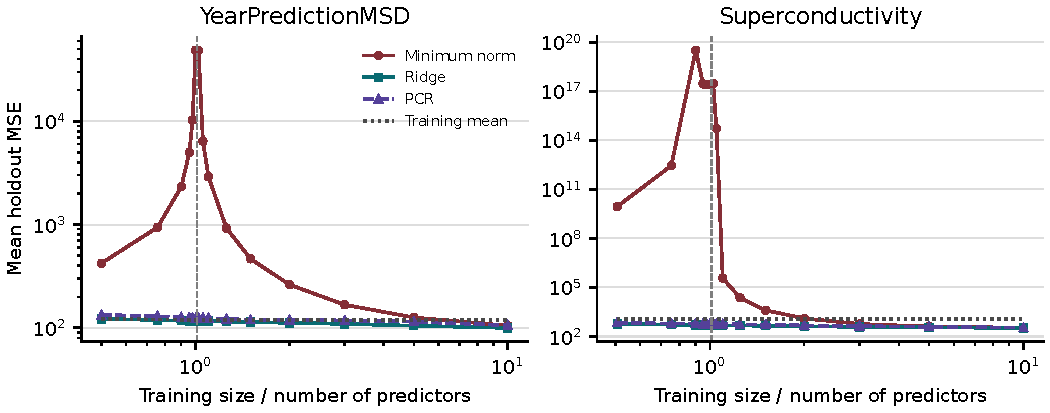
\includegraphics[width=.96\linewidth]{../replication/summary/curves.pdf}
\caption{Mean squared holdout error across 100 training prefixes at each size. Both axes use logarithmic scales. The vertical line marks the nominal centered boundary. The response units differ between panels.\FigureProvenance}
\label{fig:curves}
\end{figure}

\textbf{Results from the frozen comparisons.}
Ridge has the smallest mean MSE of the three fitted estimators at every size in both panels of Figure~\ref{fig:curves}. All 30 pointwise paired intervals for PCR minus ridge have positive lower limits. On music at $n=90$ this difference is 7.42 squared years (95\% interval 5.21 to 9.63). Ridge reduces the training-mean reference MSE from 119.21 to 115.78, a 2.9\% reduction. At $n=900$, the respective losses are 117.92 and 99.50. On materials at $n=73$, ridge scores 509.82 compared with 610.22 for PCR and 1,160.67 for the training mean. At $n=810$, minimum norm and ridge score 341.26 and 333.63, giving a paired difference of 7.63 (5.88 to 9.38).

The agreement on the regularized methods masks a difference in how the unregularized means arise. On music at $n=90$ the worst repetition contributes 25.1\% of the minimum-norm loss. On materials at $n=73$, repetition 5 alone contributes 99.92\%. The median there is $1.40\times10^6$, against a mean of $3.24\times10^{19}$. The median curve peaks at $n=81$. At eight materials sizes from 41 through 85, ridge wins all 100 paired comparisons yet the Student intervals for the mean minimum-norm excess over ridge contain zero. For example, at 73 the interval is $[-3.18,9.66]\times10^{19}$. The win fraction measures frequency and the mean measures magnitude. With only 100 draws, inference for the latter depends heavily on the sampled upper tail.

\section{Changing the numerical rank}
The worst materials prefix contains 72 distinct feature vectors in 73 rows. Its largest singular value is 47.94, its smallest retained value is $7.71\times10^{-12}$, and its default cutoff is $8.62\times10^{-13}$. The last retained direction carries more than 99.9999\% of the squared coefficient norm. These observations motivated two post-hoc checks. Both use the original data, splits and seeds. Neither benchmark was used to select a cutoff for deployment.

\subsection{Recomputing predictions on the same rows}
For each of the 1,500 materials prefixes, we keep the original preprocessing and solver and retain the singular values exceeding
\[
    \tau_c=\max(\tau_0,c s_1),\quad c\in\{0,10^{-12},10^{-10},10^{-8},10^{-6}\}.
\]
For every cutoff we restore the intercept and score the resulting predictions on all 4,392 held-out rows. This changes the estimator for affected prefixes and keeps all 100 repetitions in each curve. The default calculation reproduces all 1,500 archived minimum-norm losses exactly on the study system. Table~\ref{tab:cutoff} reports all five specifications, including settings for which the peak moves back toward smaller $n$.

\begin{table}[htb]
\centering
\caption{Materials sensitivity across the full grid. The changed count is relative to the default among 1,500 fits. Peak locations maximize the indicated sample summary over the 15 observed sizes. The last column measures concentration at the mean peak.}
\label{tab:cutoff}
\begin{tabular}{lrrrrr}
\toprule
Relative floor $c$ & Changed & Mean peak $n$ & Peak mean MSE & Median peak $n$ & Largest share\\
\midrule
\tableinput cutoff_rows.tex
\bottomrule
\end{tabular}
\end{table}

At $c=10^{-12}$ only repetition 5 changes at $n=73$. Its MSE falls from $3.24\times10^{21}$ to $2.64\times10^{15}$. The other 99 losses at that size are identical. The mean drops from $3.24\times10^{19}$ to $2.69\times10^{16}$ and the median stays at $1.40\times10^6$. Across the full grid the highest mean moves to $n=83$, on the other side of $p+1=82$. By comparison, at $c=10^{-8}$ the two highest means at $n=73$ and 81 differ by less than 0.1\%. Figure~\ref{fig:cut} shows both the size of the vertical change and the fragility of the horizontal ordering. Even after imposing the largest floor, the peak mean MSE is above $4\times10^7$.

Deleting one entire training trajectory at a time keeps the pairing across sizes. At the default cutoff, 99 deletions leave the mean peak at 73 and one moves it to 83. At $c=10^{-10}$ all 100 deletions leave the peak at 81. On comparing the two sizes singled out by the first change of cutoff, the default paired mean difference $L_{73}-L_{83}$ is $3.21\times10^{19}$, with a descriptive pointwise interval of $[-3.19,9.61]\times10^{19}$. At $c=10^{-12}$ it is $-1.55\times10^{17}$, with interval $[-4.49,1.40]\times10^{17}$. The sign reversal describes the finite archive. Neither interval resolves an ordering of the two permutation expectations, and the sizes were chosen after inspecting the curves.

\begin{figure}[htb]
\centering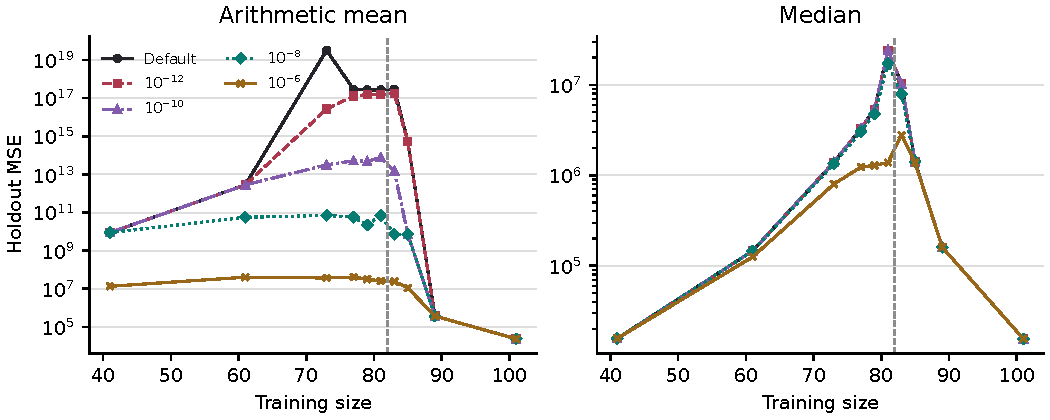
\includegraphics[width=.96\linewidth]{../replication/summary/cutoffs.pdf}
\caption{Recomputed minimum-norm losses on the materials holdout. The near-boundary part of the grid is expanded horizontally. Overlapping lines indicate identical or similar loss summaries. The vertical line marks $p+1=82$.}
\label{fig:cut}
\end{figure}

\subsection{Was the training matrix exactly singular?}
A floating-point SVD alone cannot establish the exact rank of a matrix of recorded decimal numbers. Let $A$ contain the original decimal features of a prefix, interpreted as rationals. Define $B$ by subtracting its first row from every other row. The rows of $B$ span the row space of the centered $A$: every centered row is a linear combination of differences, and subtracting two centered rows recovers their difference. Column scaling by nonzero factors preserves rank. With $m$ distinct decimal rows, $u=\min(p,m-1)$ is therefore an upper bound on the centered rank.

For a lower bound we reduce each rational entry modulo the prime $q=1{,}000{,}000{,}007$ and perform Gaussian elimination on the row differences over $\mathbb F_q$. Finite decimal denominators have only prime factors 2 and 5, so reduction is defined. A nonzero minor modulo $q$ implies a nonzero rational minor. The field rank $\ell$ is consequently a deterministic lower bound, and $\ell=u$ certifies the rank exactly. An inconclusive bound would require further work. This check uses only the printed features.

We applied it to every prefix with a default-retained singular value below $10^{-10}s_1$. There were 25 such fits across eight distinct permutations. All 25 bounds met. In 21 fits the default numerical rank equaled the certified rank. In four it was one smaller. For the worst prefix both bounds are 71 and the default fit retained 71 directions. Raising the floor to $10^{-12}s_1$ leaves rank 70. The published decimals therefore support 71 independent centered directions even though retaining the last one is disastrous for prediction. This rank result gives neither the exact magnitude of the smallest singular value nor the precision of the underlying materials measurements.


\section{Interpretation and scope}
The default curve on materials would suggest that the most difficult size lies below the nominal interpolation boundary. Recomputing just five rank-changing fits shifts the largest sample mean to the other side. The median, the largest-repetition share and the paired intervals explain different features of this change. A median peak at 81 indicates that typical fits also deteriorate near the boundary. The share of 99.92\% identifies the draw that controls the mean at 73. The exact-rank check explains why eliminating a direction can improve predictions even when that direction is present in the input as recorded.

The music data give a comparison under the same estimator definitions. Its default mean minimum-norm loss at $n=90$ is 48,972, close to 48,729 at $n=92$. The median peaks at 90. Among the 700 archived music spectra at $n\in\{81,86,88,90,92,95,99\}$, the smallest retained singular value exceeds $4\times10^{-5}s_1$ in every fit. All four alternative floors would preserve the selected directions in this window. Common vulnerability to statistical ill-conditioning can therefore coexist with very different sensitivity to the numerical floor. The source pools, feature designs and holdout constructions all differ, which prevents attribution to distribution shift.

Each arm has one fixed evaluation sample. The intervals describe draws from its source pool and have no simultaneous coverage guarantee. The peak locations describe the measured grids. Finite draws can miss rare designs and both grids omit $p+1$. Inner-fold duplicate overlap limits interpretation of the materials tuning comparison. The tolerance analysis was prompted by observed losses, and the decimal certificates apply to the selected recorded prefixes. Evaluating these diagnostics on fresh data would test their prevalence. For a reported peak, the audit that proved informative here is compact: give its largest-repetition share, show the corresponding median curve, and rescore identical prefixes across declared numerical tolerances.


\paragraph{Data and code.} The release includes paired losses for 3,000 prefixes, training seeds, 7,500 sensitivity scores, rank bounds, and scripts for the figures and paired intervals. Both original run manifests are identified by checksum. Instructions accompany the public data replay.
\url{https://github.com/fightforbelief/ood-spectral-regularization}

\paragraph{Declarations.} The authors received no specific funding for this work and declare no competing interests.

\begin{thebibliography}{9}\small
\bibitem{hastie} T. Hastie, A. Montanari, S. Rosset and R. J. Tibshirani (2022). Surprises in high-dimensional ridgeless least squares interpolation. \emph{Annals of Statistics} 50, 949--986. \href{https://doi.org/10.1214/21-AOS2133}{doi:10.1214/21-AOS2133}.
\bibitem{nakkiran} P. Nakkiran, P. Venkat, S. Kakade and T. Ma (2021). Optimal regularization can mitigate double descent. \emph{ICLR}. \url{https://arxiv.org/abs/2003.01897}.
\bibitem{hansen} P. C. Hansen (1998). \emph{Rank-Deficient and Discrete Ill-Posed Problems}. SIAM. \href{https://doi.org/10.1137/1.9780898719697}{doi:10.1137/1.9780898719697}.
\bibitem{tang} S. Tang, J. Wu, J. Fan and C. Jin (2025). Benign overfitting in out-of-distribution generalization of linear models. \emph{ICLR}. \url{https://arxiv.org/abs/2412.14474}.
\bibitem{year} T. Bertin-Mahieux (2011). Year Prediction MSD. UCI Machine Learning Repository. \url{https://archive.ics.uci.edu/dataset/203/yearpredictionmsd}.
\bibitem{super} K. Hamidieh (2018). A data-driven statistical model for predicting the critical temperature of a superconductor. \emph{Computational Materials Science} 154, 346--354. \href{https://doi.org/10.1016/j.commatsci.2018.07.052}{doi:10.1016/j.commatsci.2018.07.052}. Data: \url{https://archive.ics.uci.edu/dataset/464}.
\end{thebibliography}

\appendix
\section{Complete primary risk curves}
\begin{center}
\small
\begin{tabular}{rrrr@{\hspace{1.1em}}rrrr}\toprule
\multicolumn{4}{c}{YearPredictionMSD} & \multicolumn{4}{c}{Superconductivity}\\
\cmidrule(lr){1-4}\cmidrule(lr){5-8}
$n$ & Min.\ norm & Ridge & PCR & $n$ & Min.\ norm & Ridge & PCR\\\midrule
\tableinput risk_rows.tex
\bottomrule\end{tabular}
\end{center}
Entries are mean squared errors over the 100 permutations at each observed sample size. All three methods use the same training and evaluation rows within each repetition. The music losses are in squared years and the materials losses in squared kelvin.

\end{document}
